\subsection{Definition}
\begin{definition}
    [Cartesian vector]
    A Cartesian vector is a way to represent a vector in mathematics, physics, and engineering by breaking it down into its directional components along a Cartesian coordinate grid. 
\end{definition}

Cartesian vector notation gives us the size and direction for the rectangular components of any vector. 
Vector with its starting point at $(0, 0)$ will be referred as a Position Vector. 

\begin{example}
    Here is an example of Cartesian vector. This is also a position vector. \\
    \begin{center}
            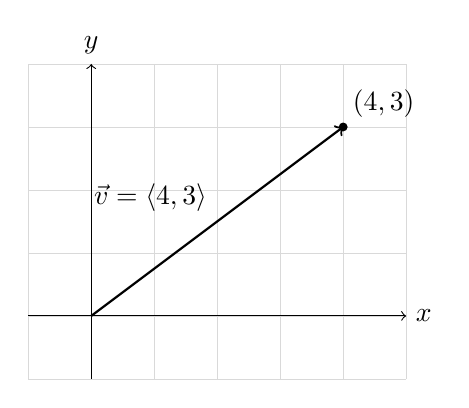
\begin{tikzpicture}[scale=0.8]
        % Grid
        \draw[step=1cm, gray!30, very thin] (-1,-1) grid (5,4);

        % Axes
        \draw[->, black] (-1,0) -- (5,0) node[right] {$x$};
        \draw[->, black] (0,-1) -- (0,4) node[above] {$y$};

        % Vector
        \draw[->, black, thick] (0,0) -- (4,3) node[midway, above left] {$\vec{v}=\langle 4,3\rangle$};

        % Point
        \fill[black] (4,3) circle (2pt) node[above right] {$(4,3)$};
    \end{tikzpicture}
    \end{center}

    In Cartesian vector notation, $\vec{v} = \left[4, 3\right]$
\end{example}



\begin{definition}
    [Magnitude of Cartesian vector]
    Given Cartesian vector $\vec{a} = \left[a_1, a_2\right]$, the magnitude of the Cartesian vector is given by 
    $$\left|\vec{a}\right| = \sqrt{
        (a_1)^2 + (a_2)^2
    }$$
\end{definition}

It is necessary to understand how to convert a geometry vector into a Cartesian vector. 

Given a geometry vector $\vec{p}$ with directoin $\theta$ degree measure from the standard position, 
this geometry vector can be converted to a Cartesian vector 
$$\vec{p} = \left[\left|\vec{p}\right|\cos \theta, \left|\vec{p}\right|\sin \theta\right]$$

\subsubsection{Property of Cartesian vector}
Given Cartesian vector $\vec{a} = \left[ a_1, a_2\right], \vec{b} = \left[b_1, b_2\right]$
\[
    \vec{a} + \vec{b} = \left[a_1 + b_1, a_2 + b_2\right]
\]
\[
    \vec{a} - \vec{b} = \left[a_1 - b_1, a_2 - b_2\right]
\]
Given a scalar $k$:
\[
    k\vec{a} = \left[ka_1, ka_2\right]
\]

We can also use the distributive property
\begin{align*}
    k\left(\vec{a} + \vec{b}\right) &= k\vec{a} + k\vec{b} \\
    &= k\left[a_1, a_2\right] + k\left[b_1 + b_2\right] \\ 
    &= \left[ka_1, ka_2\right] + \left[kb_1, kb_2\right]\\
    &= \left[ka_1 + kb_1, ka_2 + kb_2\right]
\end{align*}

For every Cartesian vector, the horizontal and vertical components can be expressed as a scalar multiples of unit vectors. 
\begin{definition}
    [Unit Vector] A vector whose magnitude is exactly 1
\end{definition}

\[
\begin{tikzpicture}[scale=2, >=Stealth]
  % Origin and endpoints
  \coordinate (O) at (0,0);
  \coordinate (I) at (1,0);
  \coordinate (J) at (0,1);

  % Axes
  \draw[aux] (-0.35,0) -- (1.45,0);
  \draw[aux] (0,-0.35) -- (0,1.45);

  % Unit vectors
  \draw[ray] (O) -- (I) node[midway, below, lab] {$\vec{i}$};
  \draw[ray] (O) -- (J) node[midway, left, lab] {$\vec{j}$};

  % Endpoint markers
  \fill[ink] (O) circle (0.8pt);
  \fill[ink] (I) circle (0.8pt);
  \fill[ink] (J) circle (0.8pt);

  % Labels
  \node[lab, below left] at (O) {$O$};
  \node[lab, below] at (I) {$(1,0)$};
  \node[lab, left] at (J) {$(0,1)$};
  \node[lab, below right] at (0.08,0) {$x$};
  \node[lab, above left] at (0,1.38) {$y$};

  % Coordinate form of basis vectors
  \node[lab, below right] at (1.05,0.2) {$\vec{i}=[1,0]$};
  \node[lab, above right] at (0.15,1.02) {$\vec{j}=[0,1]$};
\end{tikzpicture}
\]
\[
\begin{array}{c|c|c}
\text{Axis} & \text{Positive Direction} & \text{Negative Direction} \\
\hline
\text{Horizontal} 
& \vec{i}=\left[1,0\right] 
& -\vec{i}=\left[-1,0\right] \\
\text{Vertical} 
& \vec{j}=\left[0,1\right] 
& -\vec{j}=\left[0,-1\right]
\end{array}
\]

Thus, all vectors can be viewed as a linear combination of unit vectors. 

\begin{example}
    Let's expressed vector $\vec{a} = \left[3, -4\right]$ as a linear combination of unit vectors. 
    \begin{align*}
        \vec{a} &= \left[3, -4\right] \\
        &= \left[3, 0\right] + \left[0, -4\right]\\
        &= 3\left[1, 0\right] + 4\left[0, -1\right] \\
        &= 3\left[1, 0\right] - 4\left[0, 1\right] \\
        &= 3\vec{i} - 4\vec{j}
    \end{align*}
\end{example}

\newpage